\section{Runtime Design}
\label{sec:system-design}
\subsection{Responsibilities and Persistent Data}
The architecture uses C4-style responsibility and boundary labels; interaction,
activity and state views use UML conventions~\cite{c4-notation,omg-uml251}.

The React web application presents professor and student workspaces. FastAPI
handlers~\cite{fastapi-docs} expose the operations, while domain services implement
ingestion, publication and tutoring. Repositories store courses, membership,
releases, conversations, messages, learner observations and autonomous goals.
SQLite is the local persistent store; uploaded artifacts use file-based storage.
Separate workers process ingestion and scheduled tutoring opportunities.
Figure~\ref{fig:responsibilities} shows this separation.

\begin{figure}[htbp]
\centering
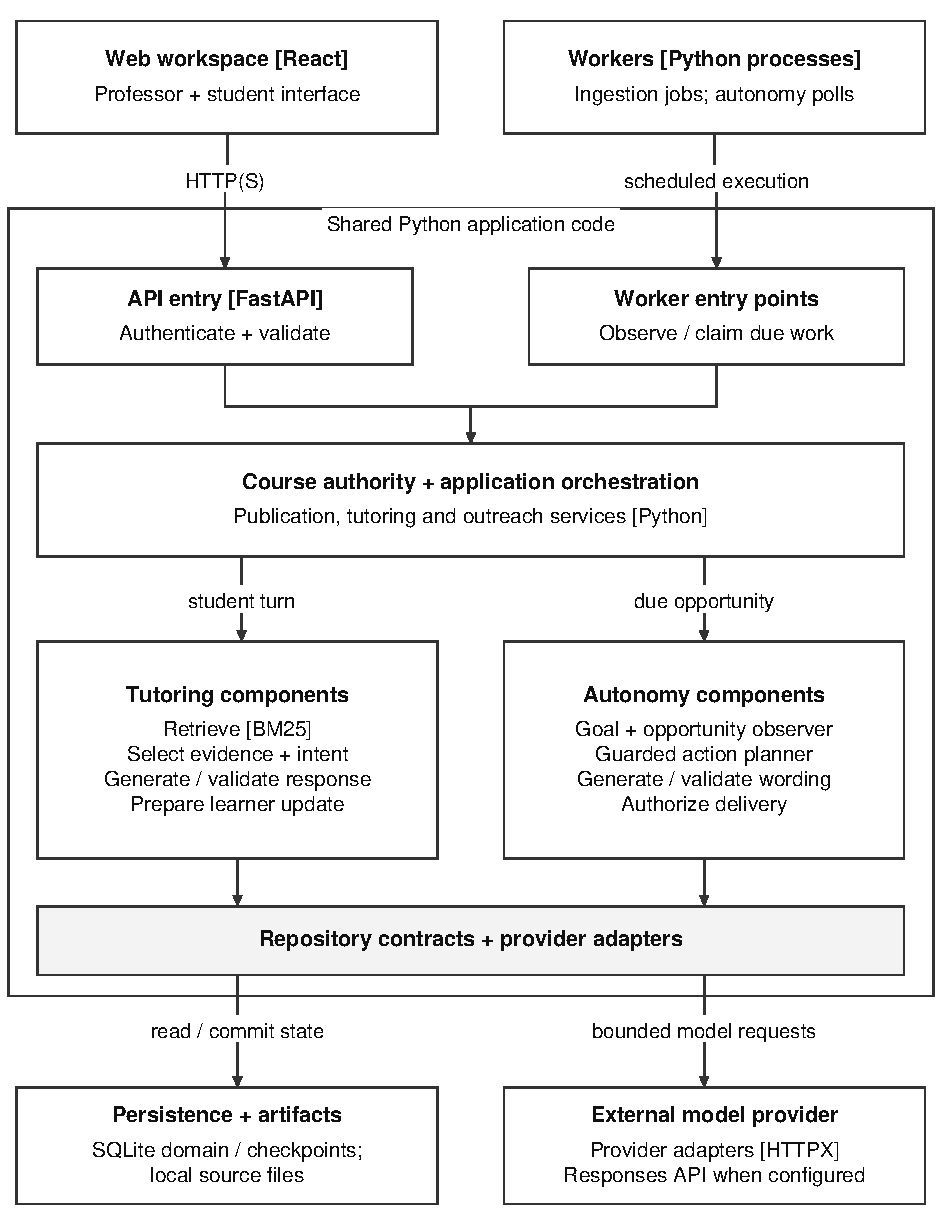
\includegraphics[width=\linewidth]{../../../reports/figures/course-twin-architecture.pdf}
\caption{Logical components shared by web requests and background workers.}
\label{fig:responsibilities}
\end{figure}

A course is owned by a professor and has student memberships. A published release
binds the policy and evidence used for tutoring. A conversation references a
course release; messages retain citations and learner observations contribute
to subsequent decisions. Autonomous goals and action outcomes also persist.
Appendix~\ref{sec:publication-data} adds publication transactions and the
conceptual persistent data model.

LangGraph provides workflow checkpoints~\cite{langgraph-docs}. Provider adapters
isolate model calls from course policy and storage. The custom OpenAI transport
uses HTTPX and the Responses API~\cite{openai-responses-docs}. Model generation
occurs outside database transactions; authority is checked again when an effect
is committed. Persisting an action requires current permission, even if a model
started generating while permission was still valid.

\subsection{From Question to Saved Response}
Figure~\ref{fig:response-sequence} traces a turn from submission to the
authorized commit of its response and learner-state update.

\begin{figure}[!ht]
\centering
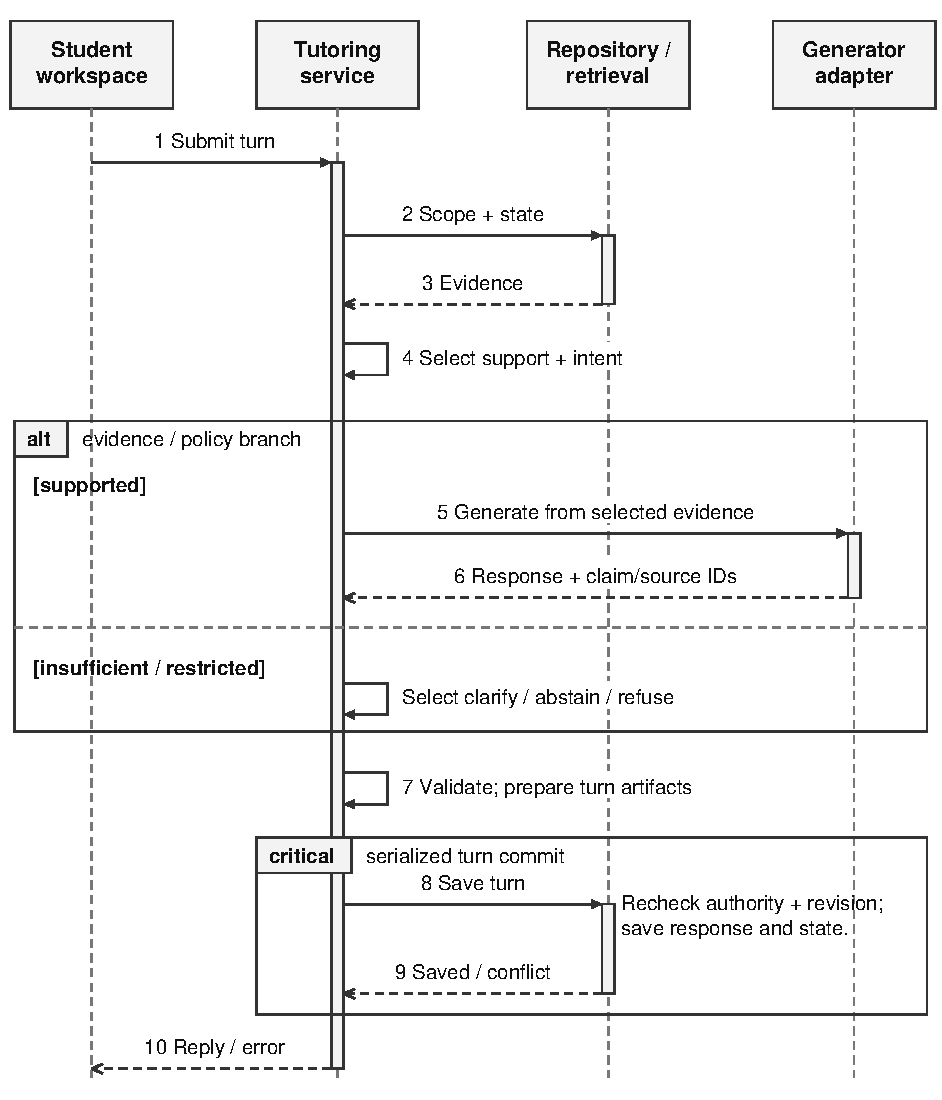
\includegraphics[width=\linewidth]{../../../reports/figures/course-twin-tutoring-sequence.pdf}
\caption{Tutoring interaction, evidence branch and serialized turn commit.}
\label{fig:response-sequence}
\end{figure}
\FloatBarrier

PyMuPDF parses approved PDFs~\cite{pymupdf-docs}; chunks preserve page boundaries,
source versions and available heading information. BM25~\cite{robertson2009bm25}
ranks eligible evidence within the student's published course. The evidence gate
checks whether support is sufficient and unambiguous. Its dominance rule
compares leading source interpretations rather than treating every weak match
as an equal competitor; competing leading answers require clarification. Retrieval and answer completeness are evaluated separately in Section~\ref{sec:grounding-comparison}.

The service validates
the account, course and release, loads policy and evidence, and invokes the
configured generation path. The retained factual path assembles approved claims
deterministically. Experimental paths ask a model for bounded explanations,
questions and feedback tied to approved source identifiers. The application
resolves citations from authoritative metadata rather than trusting invented
model links.



\begin{samepage}
After generation, current authority is rechecked within the commit boundary.
If membership, consent where applicable, or release availability has changed,
the proposed effect cannot be saved as an authorized delivery. Successful turns
persist the response, citations and associated state. A request identifier
allows matching retries to reuse the saved turn; changed content under the same
identifier is a conflict. Optimistic learner-state revision checks prevent a
stale turn from silently overwriting newer evidence.
\end{samepage}

\FloatBarrier
\subsection{From an Attempt to a Learner Record}
\label{sec:learner-state}
The observation pipeline separates identifying a concept from assessing an
answer. A turn can mention several concepts, but the primary-concept rule assigns
its assessment only to one unambiguous target; tied or weak attribution remains
unassessed. A mention therefore need not count as a correct or incorrect attempt.
The committed observation retains its concept identifiers, assessment outcome,
source references and course/release scope.

Figure~\ref{fig:learner-state} distinguishes the two consumers of stored activity.
Completion uses assessed student evidence; the default planner uses the much
simpler job-snapshot proxy. Their fields are not interchangeable.

\begin{figure}[htbp]
\centering
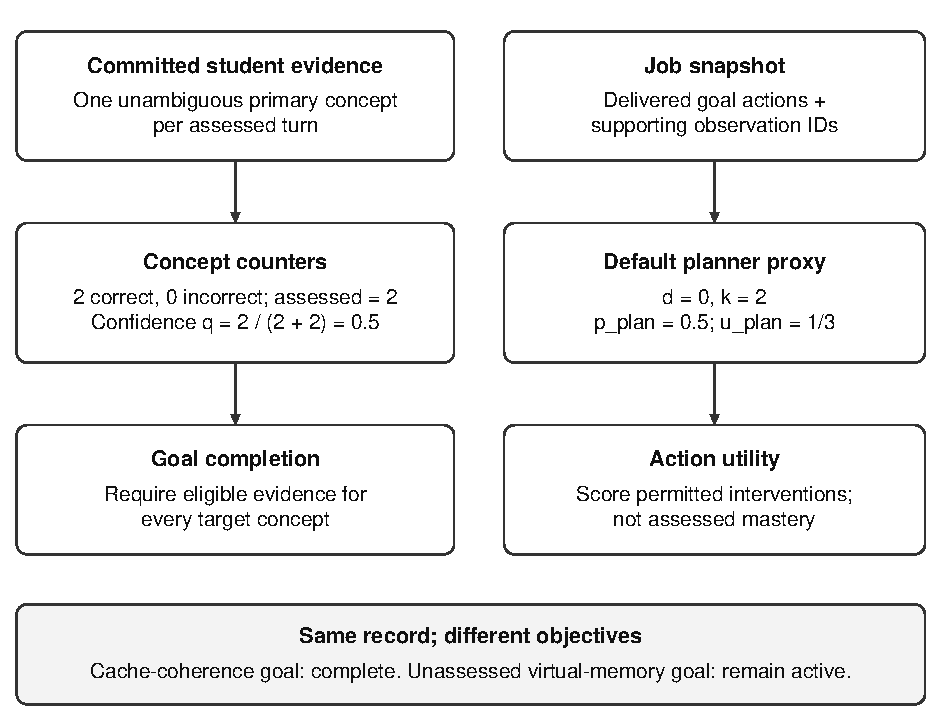
\includegraphics[width=\linewidth]{../../../reports/figures/course-twin-learner-state.pdf}
\caption{Assessment evidence and the default planner proxy have separate consumers.}
\label{fig:learner-state}
\end{figure}
For concept $c$, the evidence-count implementation records total observations,
assessed observations $a_c$, and correct, partial and incorrect counts
$(n_c^+,n_c^\sim,n_c^-)$. On an eligible assessed observation, only the relevant
outcome counter increases. Its confidence field is
\begin{equation}
q_c=\min\!\left(0.95,\frac{a_c}{a_c+2}\right).
\label{eq:evidence-confidence}
\end{equation}
Two assessed attempts give $q_c=0.5$ regardless of whether they were correct.
Thus this field represents accumulated assessment evidence, not the probability
that the student has mastered the concept. A new revision and its delta are
saved together with the accepted turn; rejected or stale observations cannot
be used as committed evidence.

The current goal correction maps each active goal $g$ to exactly one objective
in the same published domain. Let $C(g)$ be that objective's nonempty concept set,
and $S_g$ indicate that the mapping and committed learner state have valid scope.
For the evidence-count learner state, completion is
\begin{equation}
\operatorname{complete}(g)=S_g\ \land\
\bigwedge_{c\in C(g)}
\left[n_c^+\geq2\ \land\ n_c^-=0\ \land\ q_c\geq0.5\right].
\label{eq:goal-completion}
\end{equation}
Missing or ambiguous mappings remain incomplete. For example, two correct
cache-coherence assessments can satisfy a cache-coherence objective but cannot
complete an unassessed virtual-memory objective. This is the boundary reproduced
in the service audit and tested after the correction (Section~\ref{sec:goal-study}).
The rule retains a limitation: an earlier incorrect count continues to block
completion in that state. It also does not parse a professor's free-text success
condition. A completed software goal is consequently a threshold decision,
not independently demonstrated mastery.

\FloatBarrier
\subsection{How the Planner Chooses a Teaching Action}
\label{sec:planning}
The event determines candidate actions and their fallback order. Repeated
confusion permits a hint/example followed by a diagnostic question; a misconception
reverses that order. An incomplete objective or inactivity permits an in-app
check-in, and due review permits retrieval practice. The application intersects
this set with the instructor's permitted actions and adds \emph{no action}.
Let the resulting set be $A$, and $a_0$ its first permitted action.

The guarded planner scores every $a\in A$ using an inspectable forward model:
\begin{equation}
U(a)=\operatorname{clip}_{[-2,2]}
\left(G(a)+0.45O(a)+F(a)+B(a)-0.9R(a)-I(a)\right).
\label{eq:planning-utility}
\end{equation}
$G$ is a heuristic immediate-gain term weighted by estimated need and spacing;
$O$ rewards obtaining another observation when uncertainty is high; $F$ adds a
bounded look-ahead term; $B$ favours a hint or diagnostic question for repeated
errors; $R$ penalizes evidence risk and repetitive check-ins; $I$ is the
action-specific interruption cost. These constants are hand-specified, not
learned causal effects. Appendix~\ref{sec:planner-math} gives the exact terms.

Let $a^*=\arg\max_{a\in A}U(a)$, breaking ties by event order, and $a_L$
be the model proposal. Table~\ref{tab:planner-rules} makes the choice explicit;
Figure~\ref{fig:planner-decision} then applies it to the worked example.
Authorization and content validation remain separate from action selection.

\begin{table}[htbp]
\centering\small
\caption{Guarded-planner decision rules.}
\label{tab:planner-rules}
\begin{tabularx}{\linewidth}{@{}Yccccc@{}}
\toprule Condition / outcome & \shortstack{No\\evidence} & \shortstack{Invalid\\proposal} & \shortstack{Not\\best} & \shortstack{Small\\gain} & Adopt \\ \midrule
Authorized evidence ready? & N & Y & Y & Y & Y \\
Proposal valid; every step permitted? & -- & N & Y & Y & Y \\
Proposal selects analytic best ($a_L=a^*$)? & -- & -- & N & Y & Y \\
Improves fallback by at least 0.04? & -- & -- & -- & N & Y \\\midrule
Selected action & None & $a_0$ & $a_0$ & $a_0$ & $a_L$ \\
\bottomrule
\end{tabularx}
\end{table}

Ordinary provider/proposal failures retain the fallback; provider-identity errors propagate
to the failure boundary. If the model proposes the fallback itself, the action
is unchanged even though model-supplied metadata may be retained.

\textbf{What state actually reaches this planner.}
The planner receives a structured state summary, called a planning-state card.
The default adapter does not connect the detailed counts above to a calibrated
estimator. With $d$ delivered goal actions and $k$ supporting observation
identifiers, it supplies
\begin{equation}
p_{\rm plan}=\min\!\left(0.95,\frac{d+1}{d+2}\right),
\qquad u_{\rm plan}=\frac{1}{k+1}.
\label{eq:planner-proxy}
\end{equation}
The field named mastery probability therefore rises from $0.5$ to $2/3$ after
one delivery even without a student answer. Its uncertainty input counts
identifiers, not necessarily assessed attempts. Repeated-error state is derived
from the event category, and elapsed-observation time is not populated by this
adapter. These are planning proxies, distinct from Equation~\ref{eq:evidence-confidence}
and the simulator's hidden mastery. The BKT/PFA comparisons in
Section~\ref{sec:timing-comparison} are experimental alternatives, not evidence
that those estimators already drive the retained application.

\textbf{A worked calculation.}
For a repeated-confusion event with both actions permitted, zero delivered goal
actions, two supporting identifiers and ready evidence, the default adapter gives
$p_{\rm plan}=0.5$, $u_{\rm plan}=1/3$ and zero goal progress. At look-ahead
depth two, the code yields $U(\text{hint})=0.325$ and
$U(\text{diagnostic question})\approx0.267$. The event fallback is already the
hint, so a model-proposed question cannot replace it. This calculation explains
the implemented rule; it is not a recorded model response or evidence that a
hint is educationally optimal.

\begin{figure}[htbp]
\centering
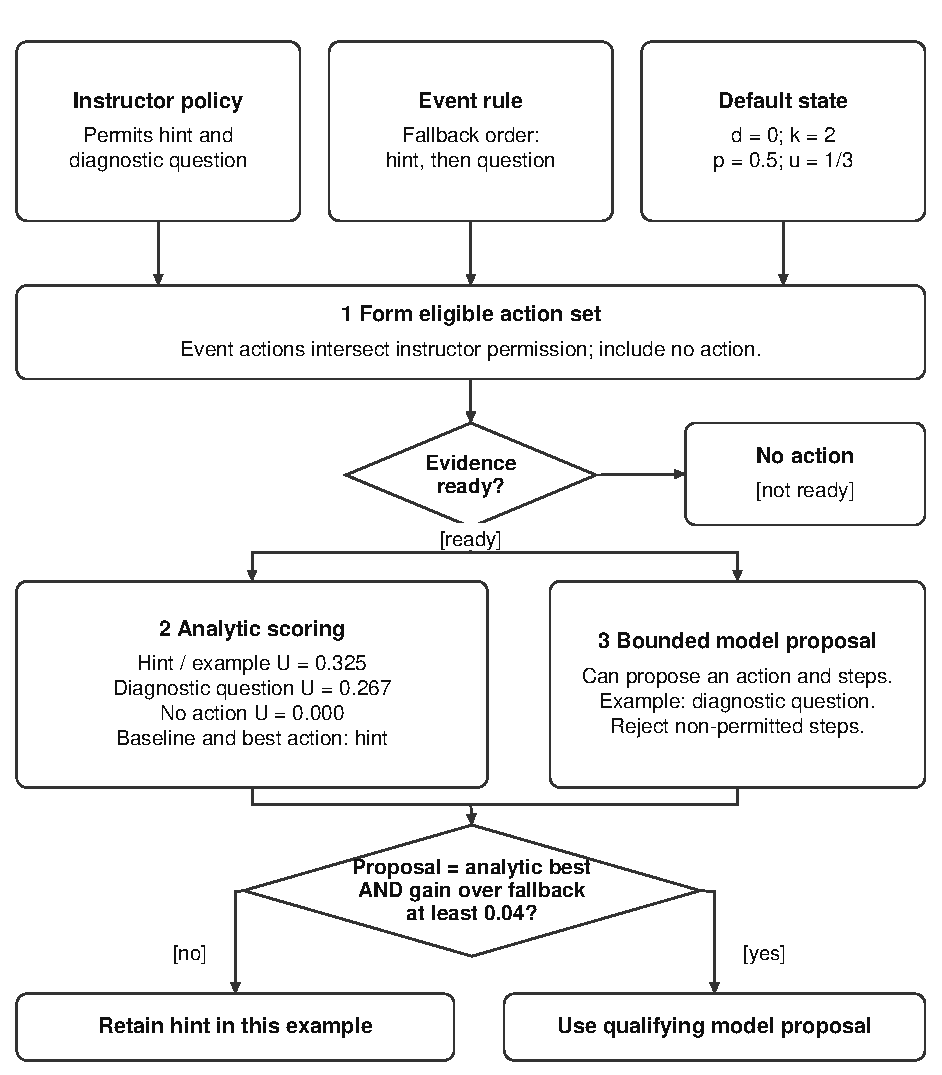
\includegraphics[width=\linewidth]{../../../reports/figures/course-twin-planner-decision.pdf}
\caption{Repeated-confusion example: the proposed diagnostic question cannot replace the higher-scoring hint.}
\label{fig:planner-decision}
\end{figure}


\FloatBarrier
\subsection{From a Durable Event to Proactive Delivery}
Autonomy here means initiating a permitted teaching action without a new
student request. A separate worker polls durable state every 30 seconds by
default. A \emph{goal} records an approved learning objective and its stopping
conditions. An \emph{opportunity} records an event, student, release and time
window in which support may be considered. An opportunity does not authorize a
message by itself.

The observer derives events from stored interactions. For example, two recent
observations with confusion scores of at least 0.7 and an overlapping concept
produce a repeated-confusion event; inactivity defaults to 72 hours without a
student message. Both thresholds are configured heuristics. Due opportunities are claimed
with a time-limited worker lease before processing.



\begin{figure}[htbp]
\centering
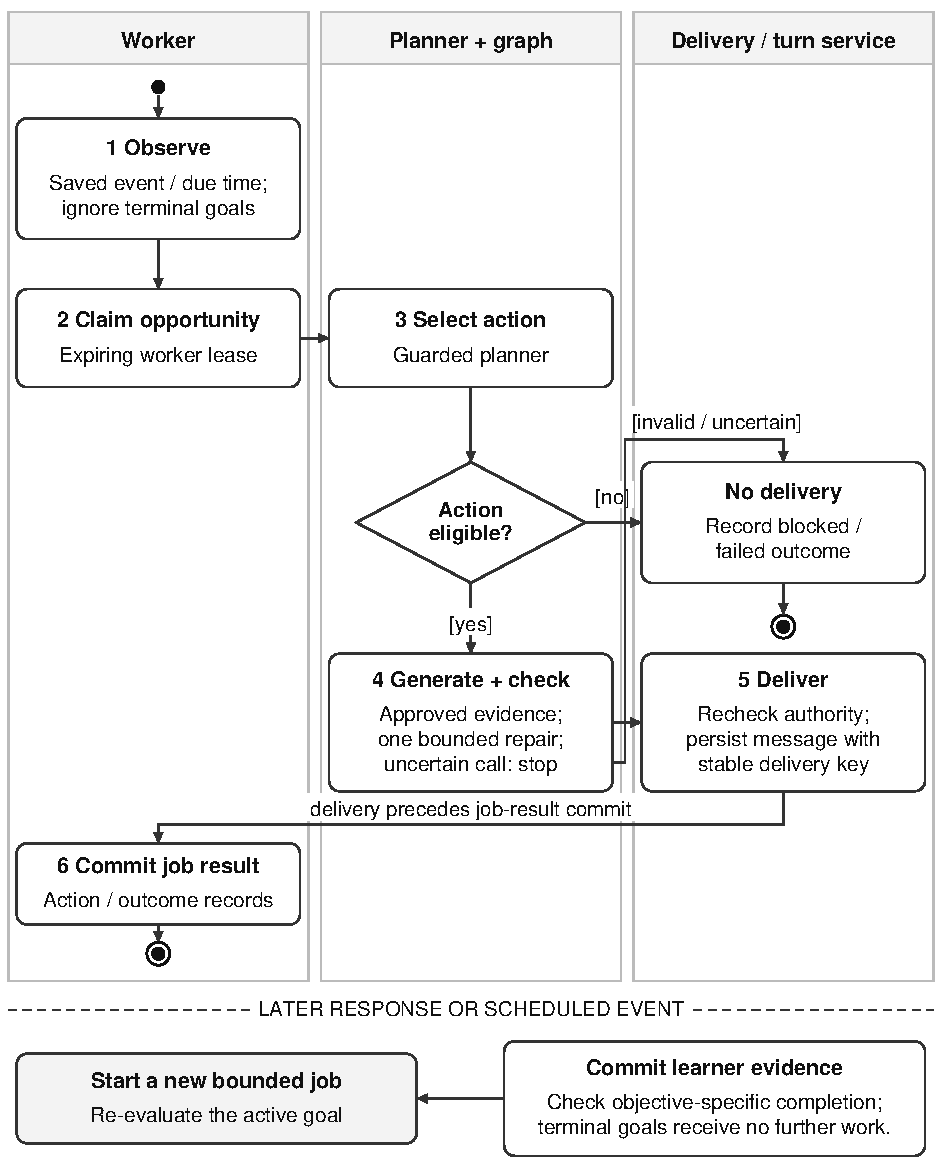
\includegraphics[width=\linewidth]{../../../reports/figures/course-twin-autonomy.pdf}
\caption{A proactive job ends after delivery or a recorded no-delivery outcome; later evidence starts another decision.}
\label{fig:autonomy}
\end{figure}

The selected model-backed wording adapter asks the model for an introduction
and a prompt strategy, then assembles permitted templates with approved source
text. Experimental instructional adapters instead generate richer questions and
explanations. 



Table~\ref{tab:outreach-decisions} specifies delivery conditions. These checks
surround a bounded graph: one proposal, initial generation and at most one repair.
An uncertain provider-call outcome stops without repeating the call. Delivery and
job-result recording are separate persistence steps; the recovery contract uses
a stable delivery key. The in-app workspace is the delivery channel.

\textbf{Following one recorded cycle.}
In the historical deterministic trace in Appendix~\ref{sec:historical-autonomy},
a diagnostic question and hint are followed by an incomplete-objective event
before the next student turn. That event leads to a permitted check-in, whose
opportunity, action and message identifiers link the decision to delivery.
Later student turns produce new learner-state revisions, and reopening the
store on virtual day 15 preserves the recorded state hash. This connects the
interaction, worker and persistence views. The trace predates the goal-completion
correction; the goal-completion regression tests that correction separately.


\begin{table}[htbp]
\centering\small
\caption{Outreach conditions and the outcome when a condition fails.}
\label{tab:outreach-decisions}
\begin{tabularx}{\linewidth}{@{}L{0.22\linewidth}Y Y@{}}
\toprule Boundary & Required condition & Otherwise \\ \midrule
Opportunity & Active and due; linked goal active and below its attempt limit & Record no action; do not generate or deliver. \\
Course authority & Consent, membership, current release/profile and instructor permission valid & Block outreach; revoked authority cannot be restored by a model proposal. \\
Schedule & Outside quiet hours; frequency and concept-cooldown checks pass & Suppress this attempt; subsequent eligible work requires a later event. \\
Evidence & Sufficient authorized support exists for the proposed action & Select no action; do not invent course evidence. \\
Generated content & Output passes the action and evidence checks & One bounded repair; stop if invalid or the provider outcome is uncertain. \\
Delivery commit & Authority still valid; stable delivery key not already saved & Reject revoked access, or reuse the already saved delivery on retry. \\
\bottomrule
\end{tabularx}
\end{table}

\subsection{A Goal Persists Across Bounded Jobs}
Figure~\ref{fig:goal-states} separates the long-lived goal from an individual
worker execution. A successful delivery increments the attempt count; it does
not complete the learning objective. The default goal manager allows three
attempts and sets expiry after seven days. The instructor may cancel a goal,
and authority changes can cancel its pending work. Pause and consent controls
prevent delivery independently of goal status. Terminal goals cannot be reactivated.

\begin{figure}[htbp]
\centering
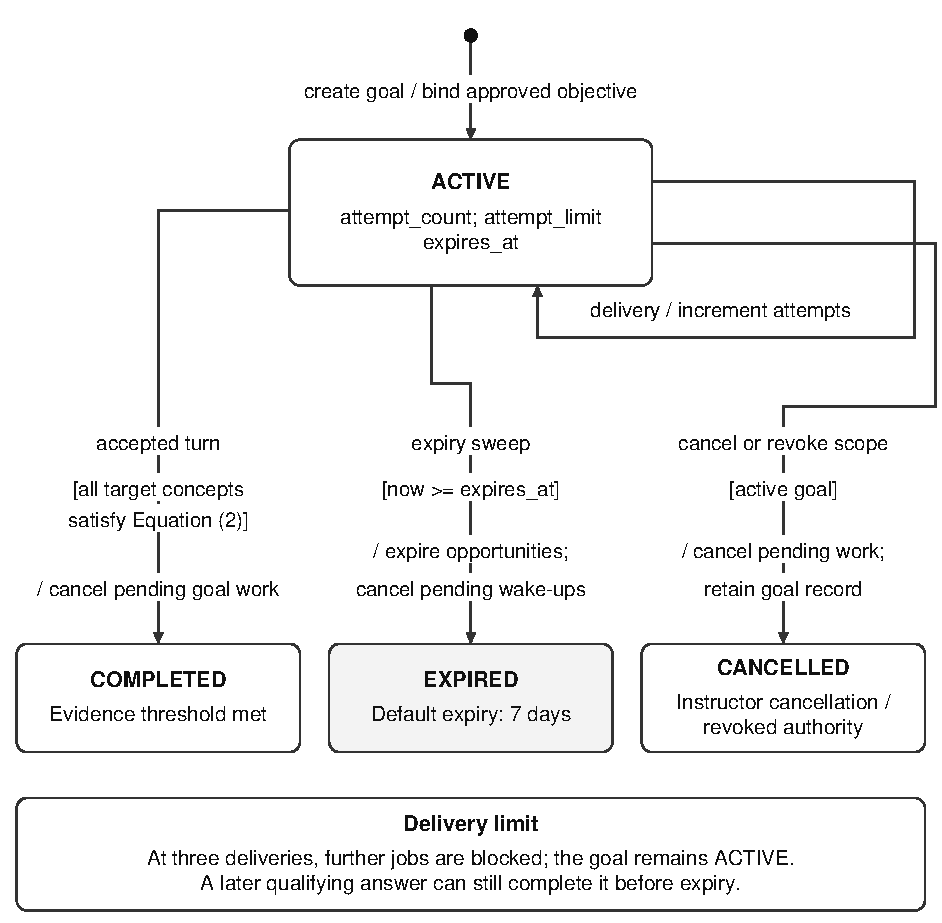
\includegraphics[width=\linewidth]{../../../reports/figures/course-twin-goal-states.pdf}
\caption{Goal transitions. Completion requires Equation~\ref{eq:goal-completion}; delivery attempts are counted separately.}
\label{fig:goal-states}
\end{figure}
